\subsection{Significance of the Photodiode: Sampling Rate, Velocity Range, and System Precision}
\label{sec:importance_bpw34_precision}

\subsubsection{Maximum Measurable Velocity with Camera}
\label{sec:camera_velocity}
Because the camera samples the irradiance waveform at $f_s = 30\text{ Hz}$, fringe skipping (temporal aliasing) occurs when the fringe-crossing rate $f_{\text{fringe}}$ becomes too fast to resolve between consecutive frames:
\begin{itemize}
    \item \textbf{Nyquist Limit for Directional Phase Tracking:} To avoid aliasing of a sinusoidally modulated signal and preserve direction reconstruction from frame samples, the fringe frequency must satisfy $f_{\text{fringe}} < \frac{f_s}{2} = 15\text{ Hz}$ (at most $\frac{1}{2}$ fringe cycle per frame). This sets the maximum velocity at
    \begin{equation}
        v_{M2, \max}^{\text{(C)}} = \frac{\lambda}{2}\,\frac{f_s}{2} = \frac{\lambda f_s}{4}
        \label{eq:vmax_nyquist}
    \end{equation}
\end{itemize}

The setup laser source has a  $\lambda = 632.8\text{ nm}$ and with the camera framrate we obtain:

\begin{equation}
    v_{M2, \max}^{\text{(C)}} \approx \frac{632.8 \times 10^{-9}\text{ m} \times 30\text{ s}^{-1}}{4} \approx 4.75 \times 10^{-6}\text{ m/s} = 4.75\ \mu\text{m/s}
\end{equation}


If mirror $M2$ moves faster than these limits, fringes cross the $\text{ROI}$ faster than the $30\text{ fps}$ frame rate can sample them, causing missed maxima/minima, underestimated displacement, and direction reversal artifacts (aliasing). Motion blur from the camera exposure time also reduces fringe contrast at higher speeds.

\subsubsection{Maximum Measurable Velocity Photodiode}
\label{sec:vmax_bpw34_fpga}

Using the PIN photodiode BPW34 (\cref{sec:PIN_Photodiode}) operated in reverse-biased mode, temporal sampling is no longer limited by a $30\text{ Hz}$ camera frame rate. Instead, fringe skipping occurs when the fringe-crossing frequency $f_{\text{fringe}}$ exceeds the effective analog bandwidth governed by the BPW34 carrier response, the TIA feedback time constant, the comparator transition, and the FPGA input-pin load, detailed in \cref{sec:circuit_schematic}.

Because the comparator outputs a single binary logic stream, direction ambiguity is not resolved from one channel alone; thus, the measurement yields unsigned fringe-crossing counts ($\Delta m \ge 0$, i.e., speed $|v_{M2, \max}|$, or signed velocity when direction is externally constrained).

A full fringe cycle requires at least one rising and one falling transition ($\sim 2 t_{\text{sw}}$), while sinusoidal attenuation in the TIA limits peak-to-peak swing above $f_{-3\text{dB}}$. Hence, the maximum resolvable fringe-crossing frequency is bounded by
\begin{equation}
    f_{\text{fringe, max}}^{(\text{PD})} \approx \min\!\left(f_{-3\text{dB}},\, \frac{1}{2 t_{\text{sw}}}\right)
    \label{eq:ffringe_max_bpw34}
\end{equation}
and, since each fringe cycle corresponds to an axial displacement of $\frac{\lambda}{2}$ for movable mirror $M2$, the maximum measurable mirror speed before fringe skipping is
\begin{equation}
    |v_{M2, \max}^{(\text{PD})}| = \frac{\lambda}{2}\,f_{\text{fringe, max}}^{(\text{PD})}
    \label{eq:vmax_bpw34_fpga}
\end{equation}

We have $f_{-3\text{dB}} \approx 6.37\text{ MHz}$, reducing its first-order $10\%\text{--}90\%$ rise/fall time to
\begin{equation}
    t_{r,\text{TIA}} = 2.2\,R_f C_f = 2.2 \times (10\,\text{k}\Omega)(2.5\text{ pF}) = 55\text{ ns}
\end{equation}
The remaining signal-path stages contribute:
\begin{itemize}
    \item \textbf{BPW34 carrier response:} $t_{r,\text{PD}} \approx 100\text{ ns}$ (representative datasheet transition time, now the dominant speed bottleneck).
    \item \textbf{TLV3542 comparator:} across a $3.3\text{ V}$ swing at $150\text{ V}/\mu\text{s}$ we obtain: \\
    $t_{\text{slew}} \approx 3.3\text{ V} / (150\text{ V}/\mu\text{s}) \approx 22\text{ ns}$.
    \item \textbf{Arty Z7-20 I/O pin load:} $R_{\text{out}} = 47\,\Omega$ in series with the board's protection resistor $200\,\Omega$ on Shield digital I/O pins, driving $C_{\text{load}} \approx 20\text{ pF}$ yields at most $t_{r,\text{pin}} \approx 2.2\,(247\,\Omega)(20\text{ pF}) \approx 10.9\text{ ns}$.
\end{itemize}
Combining all four stages by root-sum-of-squares gives the total front-end switching time:
\begin{equation}
    t_{\text{sw}} \approx \sqrt{t_{r,\text{TIA}}^2 + t_{r,\text{PD}}^2 + t_{\text{slew}}^2 + t_{r,\text{pin}}^2}
    \approx \sqrt{55^2 + 100^2 + 22^2 + 10.9^2}\text{ ns} \approx 117\text{ ns}
\end{equation}
Because the TIA bandwidth ($6.37\text{ MHz}$) now exceeds the switching-time limit, the maximum resolvable fringe frequency is governed by $\frac{1}{2 t_{\text{sw}}}$:
\begin{equation}
    f_{\text{fringe, max}}^{(\text{PD})} \approx \frac{1}{2 \times 117\text{ ns}} \approx 4.27\text{ MHz}
\end{equation}
For a red laser at $\lambda = 632.8\text{ nm}$, the corresponding maximum measurable mirror speed is:
\begin{equation}
    |v_{M2, \max}^{(\text{PD})}| \approx \frac{632.8 \times 10^{-9}\text{ m}}{2 \times 1} \times 4.27 \times 10^6\text{ Hz} \approx 1.35\text{ m/s}
\end{equation}

\subsubsection{System Precision}

Integrating the reverse-biased BPW34 photodiode and the FPGA counter transforms the interferometer from a quasi-static imaging setup into a high-speed metrological instrument. While the camera captures two-dimensional interference patterns, its $33.3\text{ ms}$ frame interval introduces motion blur and limits fringe tracking speed. By collapsing detection to a fast single-point photodetector sampled continuously in programmable logic on the FPGA, the photodiode setup overcomes this temporal bottleneck in three critical ways:

\begin{itemize}
    \item \textbf{Higher Effective Sampling Rate:}
    Instead of integrating photons over tens of milliseconds, the photodiode setup converts optical irradiance variations into real-time digital voltage swings with a combined rise time of $t_{\text{sw}} \approx 117\text{ ns}$.

    \item \textbf{Velocity Measurement:}
    Raising the maximum fringe-crossing frequency from $15\text{ Hz}$ to $4.27\text{ MHz}$ extends the measurable mirror speed for $\lambda = 632.8\text{ nm}$ from $4.75\ \mu\text{m/s}$ up to $|v_{M2, \max}^{(\text{PD})}| \approx 1.35\text{ m/s}$, an expansion of nearly $3 \times 10^5$. This dynamic range allows the interferometer to track motorized linear actuators, rapid transient displacements, and high-frequency mechanical vibrations without fringe skipping. Moreover, because the FPGA can latch a free-running $8\text{ ns}$ timestamp counter on each incoming edge, instantaneous mirror speed can be reconstructed on a per-fringe basis via $|v_{M2}(t)| = \frac{\lambda}{2\,\Delta t}$, where $\Delta t$ is the measured period between consecutive fringe transitions.

    \item \textbf{Sub-Micrometer Spatial and Nanosecond Temporal Precision:}
    The overall precision of the system arises from the combination of optical interferometric resolution, clean analog conditioning, and synchronous digital capture:
    \begin{enumerate}
        \item \textit{Optical quantization:} Each complete fringe cycle corresponds to a mirror displacement of $\frac{\lambda}{2} = 316.4\text{ nm}$ (or $\frac{\lambda}{4} = 158.2\text{ nm}$ when the FPGA edge detector counts both rising and falling transitions), providing intrinsic nanometer-scale displacement without requiring analog-to-digital amplitude interpolation.
        \item \textit{Temporal quantization:} At a $125\text{ MHz}$ FPGA clock, timing jitter due to digital sampling is negligible across typical mechanical speeds. For example, at a mirror velocity of $10\text{ mm/s}$ ($f_{\text{fringe}} \approx 31.6\text{ kHz}$, $T_{\text{fringe}} \approx 31.6\,\mu\text{s}$), the $8\text{ ns}$ clock resolution corresponds to a relative timing precision of roughly $0.025\%$ per fringe period.
        \item \textit{Noise Reduction:} Operating the TIA just above critical damping ($C_f = 2.5\text{ pF} > C_{f,\min}$) avoids ringing on fast optical transients, while the $150\text{ mV}$ Schmitt-trigger hysteresis band avoids unwanted digital changes when crossing the voltage thresholds.
    \end{enumerate}
\end{itemize}

In summary, whereas a camera excels at capturing two-dimensional spatial fringe geometry for static wavefront inspection, the \textbf{BPW34} + \textbf{TLV3542} + \textbf{Arty Z7-20} setup provides the high temporal bandwidth, wide velocity ceiling, and noise-resilient nanosecond precision needed for real-time dynamic displacement and speed metrology (with direction either externally constrained or inferred from known actuator trajectories).


\section{Digital Pulse Integrity Validation via LED PWM}
\label{sec:led_pwm_validation}

To validate the complete FPGA DAQ chain:  photodiode, TIA and Schmitt trigger, FPGA input and ComBlock memory interface prior to interferometer measurements, a controlled pulsed-light characterization was conducted using a red LED ($625\text{--}660\text{ nm}$) driven by an ESP32 hardware timer burst sweep. The FPGA sampled the digitized comparator output continuously at $f_s = 50\text{ MHz}$ ($\Delta t = 20\text{ ns}$). Characterization was evaluated across eleven frequency steps spanning more than four orders of magnitude, from $100\text{ Hz}$ up to $2\text{ MHz}$ (\cref{fig:led_pwm_sweep} and \cref{tab:led_pwm_results}).



\begin{table}
\centering
\caption{Summary of FPGA-measured pulse metrics across the LED PWM sweep ($f_s = 50\text{ MHz}$).}
\label{tab:led_pwm_results}
\begin{tabular}{cccccc}
\hline
$f_{\text{set}}$ & $f_{\text{meas}}$ & Pulses ($N$) & Missed & Duty Cycle & $\sigma_T$ [ns] \\
\hline
$100\text{ Hz}$  & $100.00\text{ Hz}$  & $40$   & $0$ & $50.00\%$ & $8.4$ \\
$500\text{ Hz}$  & $500.00\text{ Hz}$  & $90$   & $0$ & $50.00\%$ & $8.6$ \\
$1\text{ kHz}$   & $1.00\text{ kHz}$   & $190$  & $0$ & $50.00\%$ & $6.7$ \\
$5\text{ kHz}$   & $5.00\text{ kHz}$   & $490$  & $0$ & $50.01\%$ & $4.6$ \\
$10\text{ kHz}$  & $10.00\text{ kHz}$  & $989$  & $0$ & $50.02\%$ & $3.8$ \\
$50\text{ kHz}$  & $50.00\text{ kHz}$  & $1981$ & $0$ & $50.10\%$ & $3.9$ \\
$100\text{ kHz}$ & $100.00\text{ kHz}$ & $1971$ & $0$ & $50.20\%$ & $4.3$ \\
$250\text{ kHz}$ & $250.00\text{ kHz}$ & $2442$ & $0$ & $50.50\%$ & $4.4$ \\
$500\text{ kHz}$ & $500.00\text{ kHz}$ & $2777$ & $0$ & $51.00\%$ & $4.4$ \\
$1\text{ MHz}$   & $1.00\text{ MHz}$   & $2803$ & $0$ & $52.00\%$ & $4.7$ \\
$2\text{ MHz}$   & $2.00\text{ MHz}$   & $3615$ & $0$ & $56.00\%$ & $6.0$ \\
\hline
\end{tabular}
\end{table}

\subsection{Variable Pulse Counts for Calibration}
The number of analyzed pulses reported in \cref{tab:led_pwm_results} is deliberately non-uniform across frequencies, governed by two experimental design criteria:
\begin{enumerate}
    \item \textbf{Scaled Burst Duration vs.\ Data Volume Trade-Off:} To keep the total multi-frequency calibration sweep within a practical bench duration while preventing memory buffer overflow during high-speed streaming, the burst duration was scaled inversely with frequency: from $500\text{ ms}$ at $100\text{ Hz}$ down to $2\text{ ms}$ at $2\text{ MHz}$. At low frequencies, a longer time window is required to accumulate enough cycles ($N \ge 40$) for statistically meaningful period estimation. Conversely, maintaining a $500\text{ ms}$ burst at $2\text{ MHz}$ would generate over one million edge transitions, needlessly increasing the CSV dataset without providing additional insight; limiting megahertz bursts to $2\text{--}10\text{ ms}$ yields $2{,}000\text{--}3{,}600$ steady-state pulses, which is more than sufficient to bound the mean frequency and jitter with high confidence.
    \item \textbf{Exclusion of Hardware Turn-On/Turn-Off Transients:} The nominal pulse counts produced by the generator (e.g., $50$ pulses at $100\text{ Hz}$, $100$ at $500\text{ Hz}$, $200$ at $1\text{ kHz}$) were trimmed by discarding the first five and last five transitions of every burst. This step isolates steady-state optical modulation from the initial timer synchronization latency of the ESP32 LEDC peripheral and the trailing turn-off edge, resulting in the reported counts.
\end{enumerate}

\begin{figure}[htbp]
    \centering
    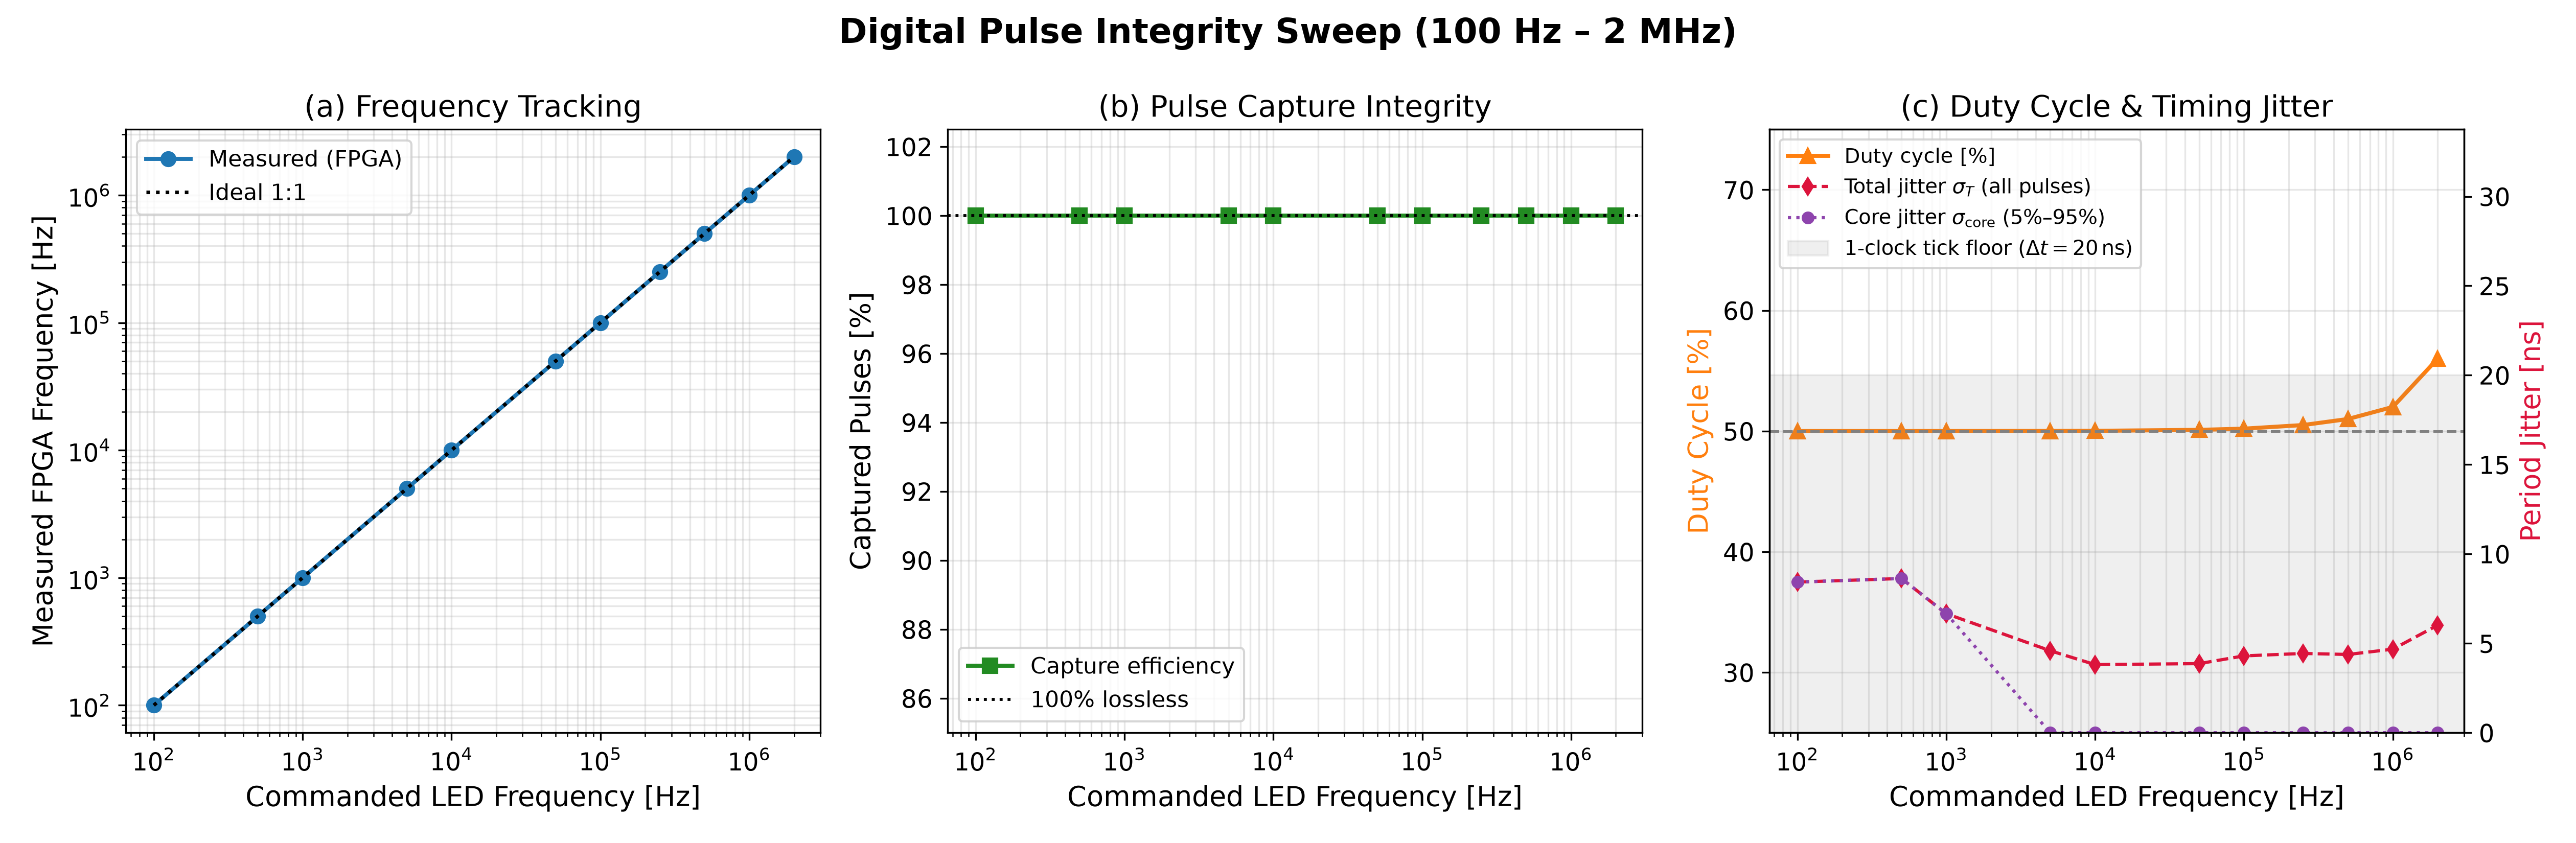
\includegraphics[width=\textwidth]{images/led_bandwidth_calibration.png}
    \caption{Digital pulse integrity validation of the FPGA DAQ ($f_s = 50\text{ MHz}$) using a pulsed red LED from $100\text{ Hz}$ to $2\text{ MHz}$: (a) frequency tracking; (b) pulse capture; (c) duty cycle stability and sub-clock period jitter.}
    \label{fig:led_pwm_sweep}
\end{figure}

\subsection{Analysis of Metrics}
The data presented in \cref{tab:led_pwm_results} and \cref{fig:led_pwm_sweep} demonstrate:
\begin{itemize}
    \item \textbf{Lossless Capture and 1:1 Frequency Tracking:} The measured frequency $f_{\text{meas}}$ matches the commanded frequency $f_{\text{set}}$ across all eleven tested steps (\cref{fig:led_pwm_sweep} a). Furthermore, the receiver captured all the pulses with zero missed events throughout the entire $100\text{ Hz}\text{--}2\text{ MHz}$ range (\cref{fig:led_pwm_sweep} b).
    
    \item \textbf{Duty Cycle Stability and Optical Turn-Off Response:} From $100\text{ Hz}$ to $10\text{ kHz}$, the digitized signal maintains an almost ideal symmetric square wave ($50.00\%\text{--}50.02\%$). As the operating frequency increases beyond $50\text{ kHz}$, the duty cycle widens gradually to $50.50\%$ at $250\text{ kHz}$ and reaches $56.00\%$ at $2\text{ MHz}$ (\cref{fig:led_pwm_sweep} c and \cref{tab:led_pwm_results}). This minor duty-cycle stretching is physical: standard LEDs exhibit a turn-off decay slightly slower than the fast electrical turn-on edge. At microsecond periods ($T = 500\text{ ns}$ at $2\text{ MHz}$), this tail remains above the comparator threshold $V_{\text{TH}}$ for an additional $\sim 30\text{ ns}$ ($\sim 6\%$ of the cycle), slightly extending the high state without causing pulse dropouts.
    
    \item \textbf{Sub-Clock Period Jitter ($\sigma_T$):} At $f_s = 50\text{ MHz}$ ($\Delta t = 20\text{ ns}$), the theoretical digital quantization floor governing a uniform-sampling edge detector is \cite[Chap 4.]{widrowQuantizationNoiseRoundoff2008}:
    \begin{equation}
        \sigma_{\text{quant}} = \frac{\Delta t}{\sqrt{6}} = \frac{20\text{ ns}}{\sqrt{6}} \approx 8.16\text{ ns}
    \end{equation}
    Across all eleven frequency steps, the measured period jitter $\sigma_T$ remains strictly bounded between $3.8\text{ ns}$ and $8.6\text{ ns}$ (\cref{fig:led_pwm_sweep} c), remaining below the single-clock period floor ($\Delta t = 20\text{ ns}$) and closely matching the theoretical quantization limit. This verifies that the BPW34 photodiode and TLV3542 Schmitt trigger (\cref{sec:circuit_schematic}) introduce negligible analog transition noise, confirming that the digital timing precision is primarily governed by the FPGA sampling clock.
\end{itemize}

\subsection{FPGA vs. Microcontroller (ESP32) for High-Speed Data Acquisition}
Although a low-cost microcontroller such as the ESP32 is well suited for generating test PWM signals and driving stepper motors, delegating high-speed pulse acquisition to the FPGA provides fundamental architectural advantages:
\begin{itemize}
    \item \textbf{Deterministic Hardware Parallelism vs.\ Interrupt Jitter:} On the FPGA, input synchronization, edge detection, and Block RAM packing execute concurrently in dedicated logic on every $20\text{ ns}$ clock cycle with zero interrupt latency. By contrast, an ESP32 relies on CPU execution shared with FreeRTOS scheduler ticks, flash-cache misses, and serial background routines. Attempting software-based GPIO sampling at megahertz rates inevitably results in non-deterministic latency and dropped edges.
    \item \textbf{Lossless Timestamping vs.\ Peripheral Bottlenecks:} While the ESP32 includes a hardware Pulse Counter (\texttt{PCNT}) capable of counting edges up to $40\text{ MHz}$, it functions only as an accumulator register: it cannot record individual edge timestamps or reconstruct instantaneous velocity profiles $v(t)$, duty cycles, or period jitter. Continuous DMA capture via the ESP32 \texttt{I2S} parallel peripheral is limited internal SRAM ($\sim 320\text{ KB}$, sustaining only milliseconds of raw data) and exhibits sample-skipping near $20\text{ MHz}$. In contrast, the Arty Z7-20, integrated with the ICTP ComBlock and PYNQ \cref{sec:comblock_API}, sustains continuous lossless $50\text{ MHz}$ acquisition buffered through FPGA BRAM into $512\text{ MB}$ of external DDR3 memory.
\end{itemize}

